%%
%% FundamentacaoTeorica.tex
%% Projeto Oficinas de Integração 3
%% Created by Leonardo Winter Pereira and Lucas Zimmermann Cordeiro on 10.03.2016
%% Copyright (C). All rights reserved
%%

\definecolor{darkRed}{rgb}{0.607843137254902, 0.1764705882352941, 0.1215686274509804}
\definecolor{lightRed}{rgb}{0.9568627450980392, 0.803921568627451, 0.7843137254901961}

\newcolumntype{C}[1]{>{\centering\let\newline\\\arraybackslash\hspace{0pt}}m{#1}}


\chapter{Fundamentação Teórica}
\label{chap:fundamentacaoTeorica}

    Para uma melhor compreensão e análise do funcionamento e princípios envolvidos em um controlador MIDI, é fundamental entendermos todos os conceitos nesse processo, bem como as características das tecnologias utilizadas na construção do protótipo e de ambos os aplicativos de controle. Assuntos, esses, que serão tratados no decorrer dessa seção.

    \section{MIDI}

        Uma vez que o projeto aqui proposto baseia-se, basicamente, no funcionamento deste protocolo e na troca de informações deste com outros dispositivos, é imprescindível um completo entendimento do mesmo.

        Esta será a mais longa seção deste capítulo, mas também a mais importante. Além disso, aqui serão citados grandes nomes utilizados como referência para este projeto, para o caso de o leitor se interessar pelos conteúdos aqui expostos e quiser se aprofundar nos mesmos.

        \subsection{O que é MIDI}

            O primeiro conceito que o leitor deve entender é o que é, de fato, o protocolo MIDI, citado repetidas vezes no capítulo anterior, mas que ainda não foi explicitado. Para tanto, serão citadas três definições deste e após, será estudado o real significado das mesmas.

            Adam Olson, do Conservatório Shenandoah, define MIDI como: \epigraph{[...] MIDI é um protocolo de controle que envia dados entre vários instrumentos musicais e sequênciadores.}{~\cite{McGuire}}

            Já David Miles Huber, autor do livro \textit{The MIDI Manual} define MIDI como: \epigraph{[...] Basicamente, MIDI é uma linguagem e especificação compatível de comunicação digital que permite múltiplos hardwares e softwares se comunicarem uns com os outros através de uma rede conectada.}{~\cite{Huber}}

            Robert Guérin, autor do livro \textit{MIDI Power!}, por sua vez, define MIDI como: \epigraph{[...] MIDI permite que músicos, engenheiros de som e iluminação, entusiastas da computação, ou qualquer outra pessoa usem computadores e instrumentos musicais eletrônicos para criar, ouvir e aprender sobre música, oferecendo uma linguagem comum que é compartilhado entre dispositivos e software compatíveis.}{~\cite{Guerin}}

            Com estas definições, pode-se perceber que MIDI é, por si só, incapaz de reproduzir som. Esta é sua maior qualidade. Seus dados podem ser gravados em um programa de software (conhecido como sequênciador) ou dispositivo de hardware, onde estes podem ser editados e transmitidos para instrumentos eletrônicos ou outros dispositivos para criar a música ou controlar qualquer parâmetro desejado. Além disso, MIDI pode ser separado em três entidades diferentes: A linguagem utilizada, também conhecida como protocolo de comunicação; a interface de hardware utilizada para transmitir e receber essas informações (tais como conectores e cabos); e os formatos de distribuição, tal como \sigla{SMF}{Standard MIDI Files} (Arquivos MIDI padrão). No decorrer deste capítulo, abordaremos separadamente cada entidade, a fim de entender como elas trabalham juntas e o porquê do MIDI funcionar tão bem, oferecendo interconectividade, flexibilidade e (em termos de tamanho de arquivo) portabilidade.

            Fundamentalmente, MIDI é uma linguagem de descrição de música em forma binária, em que cada palavra binária descreve um evento de uma música. Cada instrumento musical realiza um som, o qual está totalmente sobre controle do músico. O músico controla o momento em que o instrumento começará a realizar um determinado som - um tecladista pressionará uma tecla, um trompetista soprará ar e um baixista puxará uma corda. Considere esta ação como o evento \textbf{Note ON}. A mensagem MIDI em si não contém o real som tocado pelo instrumento, mas sim a ação de tocar uma determinada nota em um determinado momento e durante um determinado período.

            Quando o músico deixa de pressionar uma tecla em seu teclado ou de puxar uma corda em seu baixo, o som pára. Com MIDI, quando tal ação é realizada, uma mensagem é enviada para essa nota, para que esta deixe de realizar som. Esta mensagem é conhecida por \textbf{Note OFF}. A figura ~\ref{fig:MIDI_Nota_ON_e_OFF} demonstra um exemplo destes dois eventos.

            \begin{figure}[H]
            	\centering
            	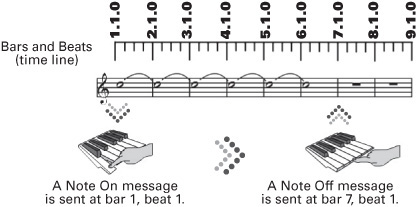
\includegraphics{Imagens/MIDI_Nota_ON_e_OFF.jpg}
            	\caption[Exemplo de transmissão das mensagens de Nota ON e OFF]{Exemplo de transmissão das mensagens de Nota ON e OFF ~\cite{Guerin}}
            	\label{fig:MIDI_Nota_ON_e_OFF}
            \end{figure}

            A fim de identificar qual nota foi ativada / desativada no instrumento, um número é atribuído para cada nota. MIDI também lida com valores interpretativos, como por exemplo a velocidade que a nota foi pressionada e a pressão que é executada na mesma.

        \subsection{O protocolo de comunicação MIDI}

            O protocolo de comunicação MIDI é transmitido de forma serial ao invés de paralela. Em uma transmissão paralela, como o nome sugere, as informações são transmitidas simultaneamente. A quantidade de dados que podem ser transmitidos simultaneamente depende na capacidade física do fio e da velocidade com que os dispositivos podem enviar suas informações. Na figura ~\ref{fig:Parallel_versus_serial_transmissions}, podemos perceber que um \textit{byte} (oito \textit{bits}) é transmitido simultaneamente utilizando uma transmissão paralela. A transmissão serial, por outro lado, consegue enviar apenas um \textit{bit} após o outro.

            \begin{figure}[H]
            	\centering
            	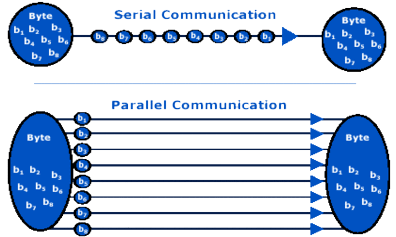
\includegraphics[scale=0.8]{Imagens/Parallel_versus_serial_transmissions.png}
            	\caption[Comparação entre transmissão serial e paralela]{Comparação entre transmissão serial e paralela}
            	\label{fig:Parallel_versus_serial_transmissions}
            \end{figure}

            A pergunta que fica é: Por que MIDI usa transmissão serial ao invés da transmissão paralela?

            A resposta para essa pergunta está no período em que o protocolo foi desenvolvido. A transmissão paralela tinha algumas desvantagens que superavam as vantagens desta sobre a transmissão serial, além de ser muito mais cara, uma vez que os fios, conectores e tomadas eram mais complexos. Já a transmissão serial, por outro lado, era muito mais simples de ser produzida, mais acessível para o público e rápida o suficiente para os fins que os fabricantes e usuários tinham em mente naquela época, para não mencionar mais confiável. Com o passar dos anos, a tecnologia avançou muito e os custos da transmissão paralela despencaram. Entretanto, para manter o MIDI compatível com todos os antigos dispositivos, sua forma de transmissão de dados permaneceu inalterada desde sua introdução no mercado.

            MIDI envia informação a uma taxa de 31250 \sigla{bps}{\textit{bits} por segundo}. Essa velocidade é chamada de taxa de transmissão. Uma vez que o protocolo utiliza transmissão serial, o mesmo envia apenas um \textit{bit} por vez. Cada \textit{byte} em uma mensagem MIDI contém 10 \textit{bits} de dados (8 \textit{bits} para as informações e 2 \textit{bits} para correção de erro). Isso significa que MIDI envia cerca de 3125 \textit{bytes} de dados cada segundo.

            Quando comparamos esse valor com a taxa de transmissão de 176400 \textit{bytes} necessária para transmitir áudio digital (reprodução e gravação) em formado de CD de áudio, MIDI pode parecer incrivelmente devagar. Entretanto, neste último não é necessário enviar tanta informação quanto o áudio digital, sendo capaz de, teoricamente, transmitir até 500 mensagens MIDI por segundo. Na realidade, leva cerca de um milésimo de segundo para transmitir uma única nota. O limiar para distinguir os eventos de som individuais é de aproximadamente 10 milissegundos, então você apresentará dificuldades com 10 ou mais eventos simultâneos.

        \subsection{Hardware e conectores}

            Informações MIDI são transmitidas através de fios e conectores, e seus cabos podem apresentar até 15 metros de comprimento. Entretanto, por se tratar de um cabo serial, todos os dados são transmitidos através de um único fio principal, e grandes distâncias podem inferir em uma degradação do sinal, ocasionando em possíveis perdas de dados ou mensagens impossíveis de serem lidas.

            \begin{figure}[H]
            	\centering
            	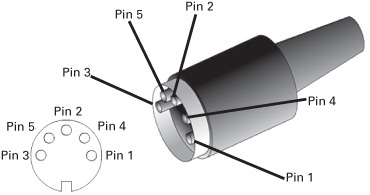
\includegraphics[scale=0.8]{Imagens/MIDI_connector.jpg}
            	\caption[Conector MIDI]{Conector MIDI}
            	\label{fig:MIDI_connector}
            \end{figure}

            O conector MIDI, semelhante ao apresentado na figura ~\ref{fig:MIDI_connector}, apresenta 5 pinos distintos. Entretanto, como já mencionado, MIDI envia informações utilizando um protocolo de transmissão serial. Desta forma, apenas um pino é realmente utilizado para o envio de informações. A tabela ~\ref{table:MIDI_pins} descreve cada pino do conector e sua respectiva função.

            \begin{center}
                \tablefirsthead{%
                  \hline
                  \rowcolor{darkRed} \textcolor{white}{\textbf{Pino}} & \textcolor{white}{\textbf{Descrição}} \\
                  \hline}
                \tablehead{%
                  \hline
                  \multicolumn{2}{|l|}{\small\sl continuação da página anterior} \\
                  \hline
                  \rowcolor{darkRed} \textcolor{white}{\textbf{Pino}} & \textcolor{white}{\textbf{Descrição}} \\
                  \hline}
                \tabletail{%
                  \hline
                  \multicolumn{2}{|r|}{\small\sl continua na próxima página} \\
                  \hline}
                \tablelasttail{\hline}
                \bottomcaption{Pinos em um conector MIDI
                \label{table:MIDI_pins}}
                %
                \begin{supertabular}{| C{0.8cm} | C{14.3cm} |}
                    \rowcolor{lightRed} 1 &  Não é utilizado. Na maioria dos cabos MIDI, este pino não está conectado a nenhum fio. \\
                    \rowcolor{white}    2 &  Este é utilizado para proteção elétrica (~\sigla{GND}{Ground}). Esta proteção impede que a transmissão apresente sinais elétricos indesejados. \\
                    \rowcolor{lightRed} 3 &  Como o Pino 1, este também não é utilizado, e na maioria dos cabos MIDI, também não está conectado a nenhum fio. \\
                    \rowcolor{white}    4 &  Este é o único receptor de dados MIDI. As informações através deste cabo fluem em uma única direção. \\
                    \rowcolor{lightRed} 5 &  Este é o único transmissor de dados MIDI e, assim como no pino 4, as informações também fluem unidirecionalmente. \\
                \end{supertabular}
            \end{center}

            Além do conector, outro hardware importante, que vale a pena ser ressaltado, é a versão fêmea do cabo MIDI. Controladores MIDI, como o desenvolvido neste projeto, apresentam normalmente 2 ou 3 destes conectores, rotulados como \textbf{In}, \textbf{Out} e \textbf{~\sigla{Thru}{Through}} (veja a figura ~\ref{fig:MIDI_connector_Female}). O conjunto destes conectores é chamado de \textbf{porta MIDI} e cada uma deles será explicado com mais detalhes a seguir.

            \begin{figure}[H]
            	\centering
            	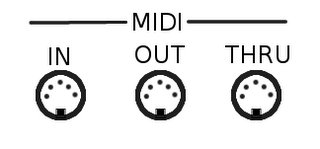
\includegraphics[scale=0.8]{Imagens/midi_in_out_thru.png}
            	\caption[Conectores fêmeas MIDI]{Conectores fêmeas MIDI}
            	\label{fig:MIDI_connector_Female}
            \end{figure}

            \begin{itemize}
                \item MIDI IN: Através deste conector são recebidas as mensagens MIDI de um determinado dispositivo ou software MIDI. Estas mensagens podem então ser processadas e, caso desejado, enviadas para outro dispositivo através do conector MIDI Thru.

                \item MIDI OUT: Através deste conector são transmitidas as mensagens MIDI que são geradas em um software ou dispositivo MIDI. Esta saída não envia informação de áudio, mas sim simples mensagens MIDI que são interpretadas por um conector MIDI In de um outro dispositivo. Tais mensagens são códigos digitais que representam o que e como músicas e eventos são tocados em um determinado instrumento.

                \item MIDI THRU: envia uma réplica do sinal recebido na porta In para o componente ligado a ele, seja em cadeia ou somente os dois, desde que sejam componentes MIDI.
            \end{itemize}

        \subsection{Formatos de distribuição}

            Como já dito no início deste capítulo, existe um formato de arquivo padrão para MIDI, o SMF. Este tipo de arquivo armazena todas as informações necessárias para reproduzir todos os parâmetros suportados pelo protocolo. Além disso, ele também adiciona o que chamamos de \textit{time stamp} em cada evento, para que o software MIDI, ou até mesmo o usuário final, saiba o momento correto de realizar cada um destes.

            MIDI tem a vantagem de ser compacto, uma vez que o som tocado por determinado instrumento não é gravado, mas sim apenas as informações de cada evento. Devido a este fato, arquivos MIDI apresentam um tamanho cerca de 300 vezes menor do que um arquivo de música atual (MP3). Entretanto, esse valor pode ser muito maior se compararmos com formatos descompactados de músicas.

            O fato de MIDI não gravar som, entretanto, pode também ser uma desvantagem. Quando o som de um determinado instrumento é gravado, o usuário tem total controle sobre o resultado final, enquanto com MIDI, este mesmo resultado depende do dispositivo ou software que será utilizado para reproduzir este mesmo som.

        \subsection{Canais MIDI}

            Quando trabalhamos com música, muitas vezes desejamos que diversos instrumentos participem da mesma composição. Com MIDI, podemos incluir instruções para cada um deles através dos chamados \textbf{canais MIDI}.

            Pense em um canal MIDI como um canal de televisão (veja a figura ~\ref{fig:midi-channels}). Um determinado instrumento conecta-se apenas a um único canal, assim como um usuário o faz em sua televisão. Isso não significa que os outros canais não estão disponíveis, mas sim que o conteúdo disponível (no nosso caso, a mensagem MIDI) foi filtrado para processar apenas o relevante para aquele canal.

            \begin{figure}[H]
            	\centering
            	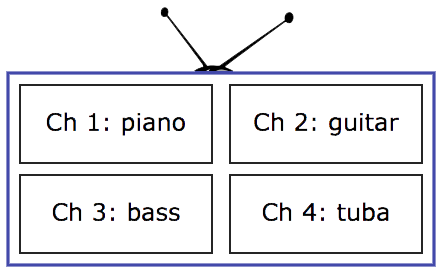
\includegraphics[scale=0.6]{Imagens/midi-channels.png}
            	\caption[Exemplo de canais MIDI]{Exemplo de canais MIDI ~\cite{Gibson2013}}
            	\label{fig:midi-channels}
            \end{figure}

            Cada porta MIDI suporta até 16 canais simultâneos. Em outras palavras, um usuário pode escolher um determinado canal para transmitir as mensagens MIDI ou possuir até 16 instrumentos conectados simultaneamente, cada um realizando diferentes eventos.

    \section{Mensagens MIDI}

        Agora que já explicamos o básico sobre o protocolo MIDI, é necessário estudarmos como podemos transmitir informações através de dispositivos. Essas informações são as chamadas \textbf{mensagens MIDI}.

        O conteúdo de uma mensagem MIDI é bastante simples. Todas elas apresentam um componente chamado de \textit{status byte}. Este componente é acompanhado por um valor que é definido por um ou mais \textit{bytes} de dados.

        Durante essa seção, os seguintes tópicos serão abordados:

        \begin{itemize}
                \item A estrutura de uma mensagem MIDI.

                \item Diferenças entre os tipos de mensagens MIDI.

                \item O que essas mensagens contêm e o que seus valores representam.

                \item Como MIDI atribui nomes e números de notas para cada evento.

                \item Como as mensagens MIDI transmitem e armazenam informações sobre a performance, e então as reproduzem no tempo correto.
        \end{itemize}

        \subsection{Mensagens de estado e de dados}

            Como já visto na seção anterior, cada \textit{byte} em uma mensagem MIDI contém 10 \textit{bits}. Destes, 8 são utilizados para a transmissão de informações. Desta forma, cada mensagem pode conter um valor entre 0 e 255. Tais mensagens são divididas em duas categorias: \textit{Estado} e \textit{Dados} (veja a figura ~\ref{fig:Status_and_Data_Bytes}).

            \begin{figure}[H]
            	\centering
            	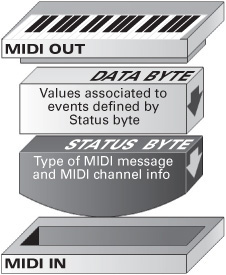
\includegraphics[scale=0.8]{Imagens/Status_and_Data_Bytes.jpg}
            	\caption[Byte de estado e de dados]{Byte de estado e de dados ~\cite{Guerin}}
            	\label{fig:Status_and_Data_Bytes}
            \end{figure}

            \begin{itemize}
                \item A porção referente ao \textit{byte} de estado serve para identificar o tipo de informação que está sendo enviada. Ela informa ao dispositivo receptor a qual canal MIDI determinado evento pertence e o que este evento é. Um evento pode ser, por exemplo, um Note On ou um Note Off. Outros eventos serão explicados no decorrer do projeto.

                \item A porção referente ao \textit{byte} de dados informa ao dispositivo receptor o valor que está associado ao evento determinado na outra porção da mensagem MIDI. Por exemplo, se o usuário decidir tocar um \textit{Dó} mediano com uma força também mediana, o \textit{byte} de estado irá enviar um evento "Note On", enquanto o \textit{byte} de dados irá passar o valor correspondente à essa nota e à velocidade que esta foi tocada. No nosso exemplo, a nota C4 tem o valor correspondente a 60 (veja a tabela ~\ref{table:MIDI_notes}) e a velocidade de aproximadamente 64.
            \end{itemize}

            Os valores utilizados pelo \textit{byte} de estado variam entre 128 e 255 (1000 0000 a 1111 1111 em números binários), enquanto para o \textit{byte} de dados estes variam entre 0 a 127 (0000 0000 a 0111 1111 em números binários). É fácil perceber que, para um dispositivo MIDI reconhecer qual o tipo de mensagem que se está sendo transmitida, basta verificar o \sigla{MSB}{Most Significant Bit} (\textit{Bit} mais significativo, do inglês). Se este valor for 1, trata-se de um \textit{byte} de estado. Caso contrário, de um \textit{byte} de dados. Simples assim.

            Digamos que um dispositivo MIDI receba três valores: 175, 43 e 125. Ele saberá que 175 é um \textit{byte} de estado, enquanto os outros dois valores são os \textit{bytes} de dados que estão acompanhando o \textit{byte} de estado. Caso este dispositivo receba outros valores, digamos: 200, 220 e 90. Ele saberá que os dois primeiros valores são \textit{bytes} de estados, enquanto o último é um \textit{byte} de dados que acompanha apenas o último \textit{byte} de estado, não ambos.

            Mensagens MIDI são normalmente representadas em um dos três mais comuns formatos digitais: decimais; binários; e hexadecimais. Explicar a conversão entre estes formatos (e os formatos em si) jazem fora do escopo deste projeto, mas podem ser consultados no livro \textit{MIDI Power!}~\cite{Guerin}.
            
            

    \section{Microcontroladores e Arduino}



        \subsection{Microcontroladores}



        \subsection{Arduino}

